\subsection{Messumgebung}

% PettingZoo-Bibliothek

Als Grundlage für die Messumgebung dient die Open Source Python-Bibliothek PettingZoo, die zum Entwickeln und Testen von MARL-Systemen konzipiert wurde. Sie stellt eine einheitliche Schnittstelle zu Umgebungen bereit, in der Agenten miteinander interagieren können.

Die Umgebungen definieren den Rahmen, in dem die Agenten miteinander interagieren. Sie weisen ein bestimmtes Verhalten auf und definieren unter anderem, unter welchen Bedingungen welche Aktionen möglich sind, Belohnungen verteilt werden und in welcher Form die Agenten Informationen über den Zustand der Umgebung erhalten. Es existieren eine Reihe von vorgefertigten Umgebungen, darunter welche, die kooperative Probleme zum Benchmarking von MARL-Systemen oder auch rundenbasierte Spiele wie Vier Gewinnt abbilden.

Die durch PettingZoo bereitgestellte Schnittstelle ermöglicht es, aus Sicht eines Agenten den aktuellen Zustand der Umgebung zu beobachten, die im aktuellen Zustand möglichen Aktionen und erhaltenen Belohnungen zu ermitteln und eine Aktion auszuwählen, die in der Umgebung durchgeführt werden soll.

Für alle Agenten der Umgebung kann benutzerdefinierte Logik eingebunden werden, die bestimmt, wie sie ihre Aktionen wählen. Vorgesehen sind dabei RL-Modelle, es können jedoch auch symbolische Algorithmen eingesetzt werden, darunter auch welche, die ihre Entscheidungen rein zufällig oder unter Einbezug von menschlichen Eingaben treffen \cite{Farama.2025}.

% Implementierung der Messumgebung

Die Implementierung der Messumgebung baut auf der offiziellen Implementierung der Vier-Gewinnt-Umgebung von PettingZoo auf. Die Messumgebung tut dabei nichts anderes, als wiederholt zwei Agenten mit bestimmten Lösungsansätzen das Spiel spielen zu lassen und dabei die Gewinnraten und Spieldauer zu messen. Die Open-Source-Eigenschaft ermöglicht es, den Quellcode zu modifizieren. Davon wird im weiteren Verlauf der Arbeit Gebrauch gemacht, unter anderem, um die verschiedenen Szenarien zur Untersuchung von Robustheit abzubilden.

Im Zuge der Realisierung der Messumgebung ist aufgefallen, dass wenn zwei Agenten (Spieler 0 und Spieler 1) alle Aktionen im Spiel mit derselben Wahrscheinlichkeit rein zufällig wählen, nach 1000 Spielen Spieler 0 mit 55,20 \% gegenüber Spieler 1 mit 44,30 \% eine wesentlich höhere Gewinnrate erzielt.

\begin{figure}[ht!]%[!tbp]
	\begin{subfigure}[b]{0.48\textwidth}
		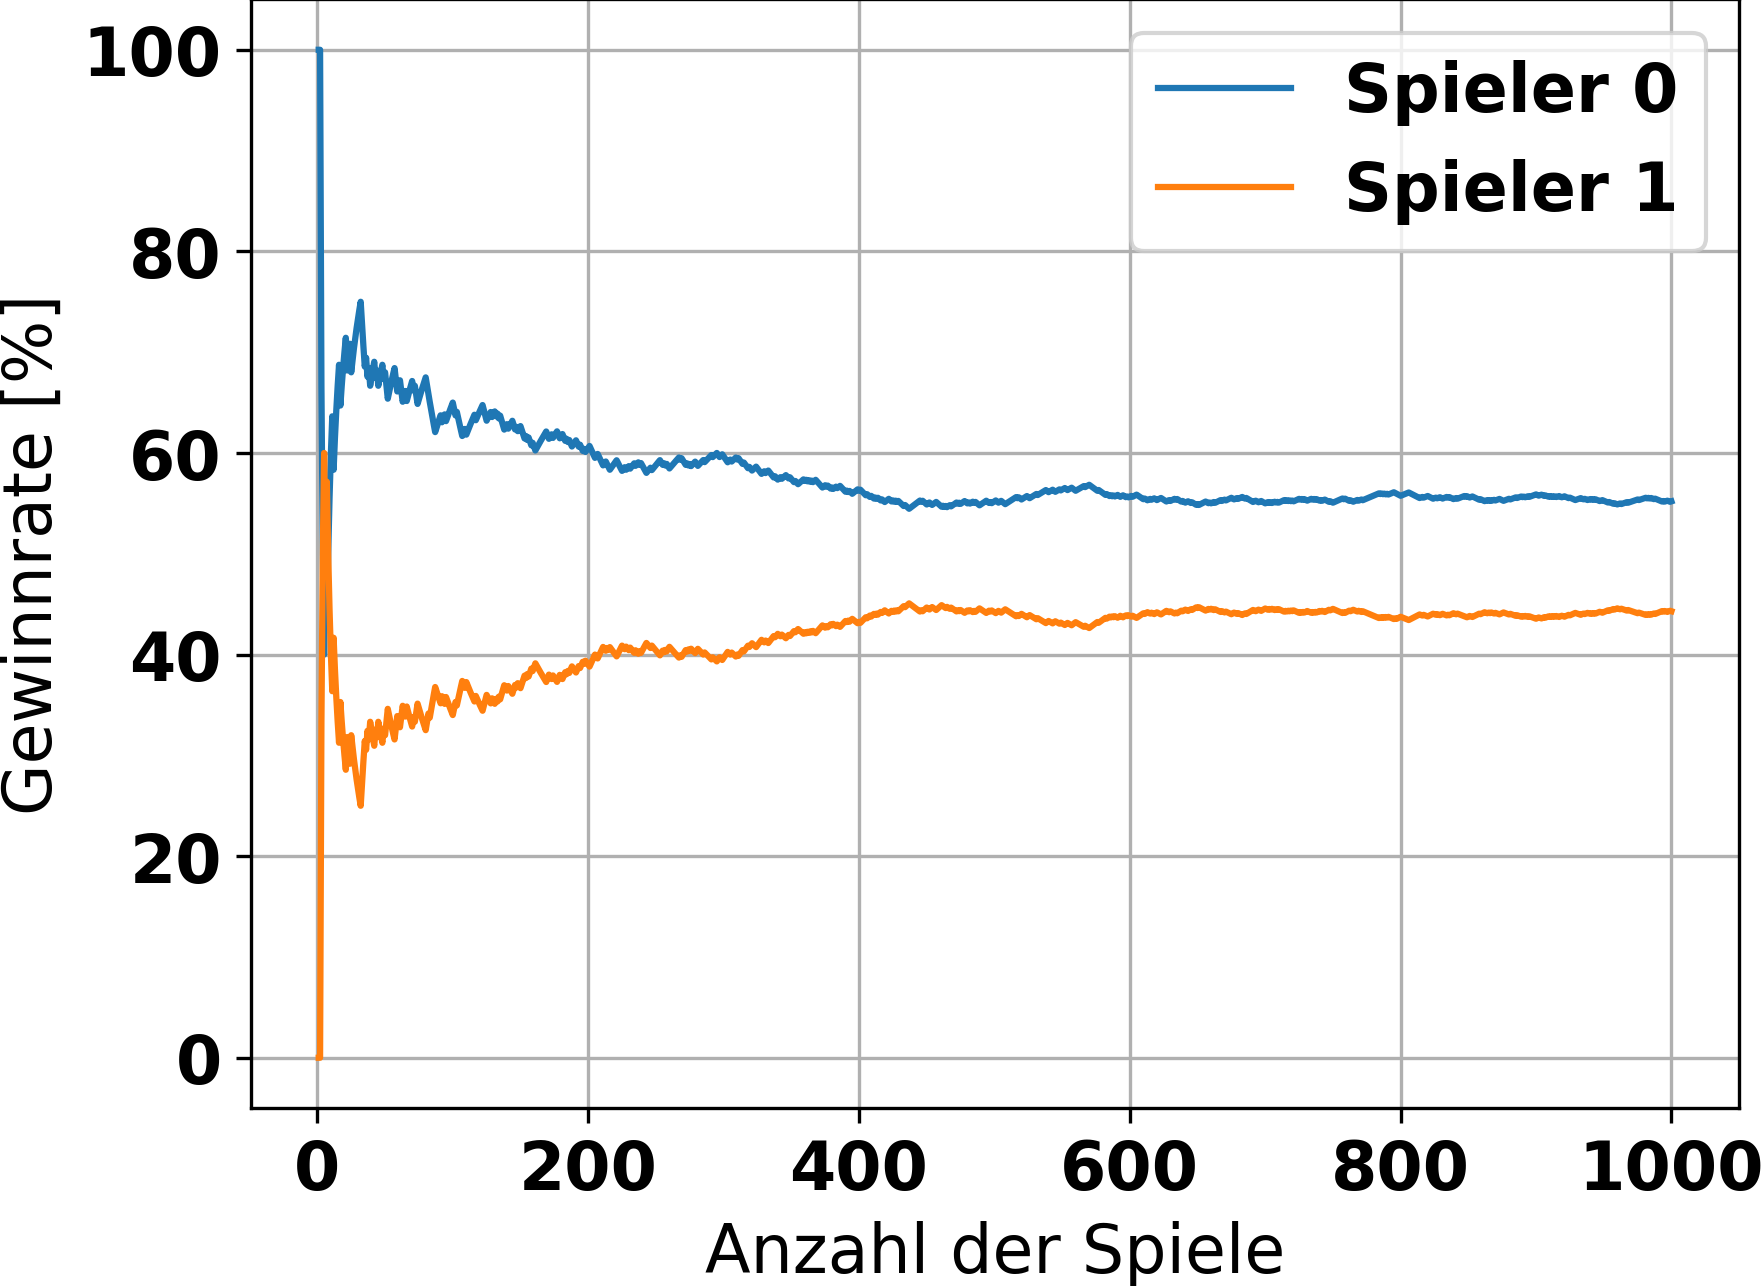
\includegraphics[width=\textwidth]{Bilder/constant_player_order_graph_win_rates.png}
		\caption{Gewinnrate.}
		\label{fig:f1}
	\end{subfigure}
	\hfill
	\begin{subfigure}[b]{0.48\textwidth}
		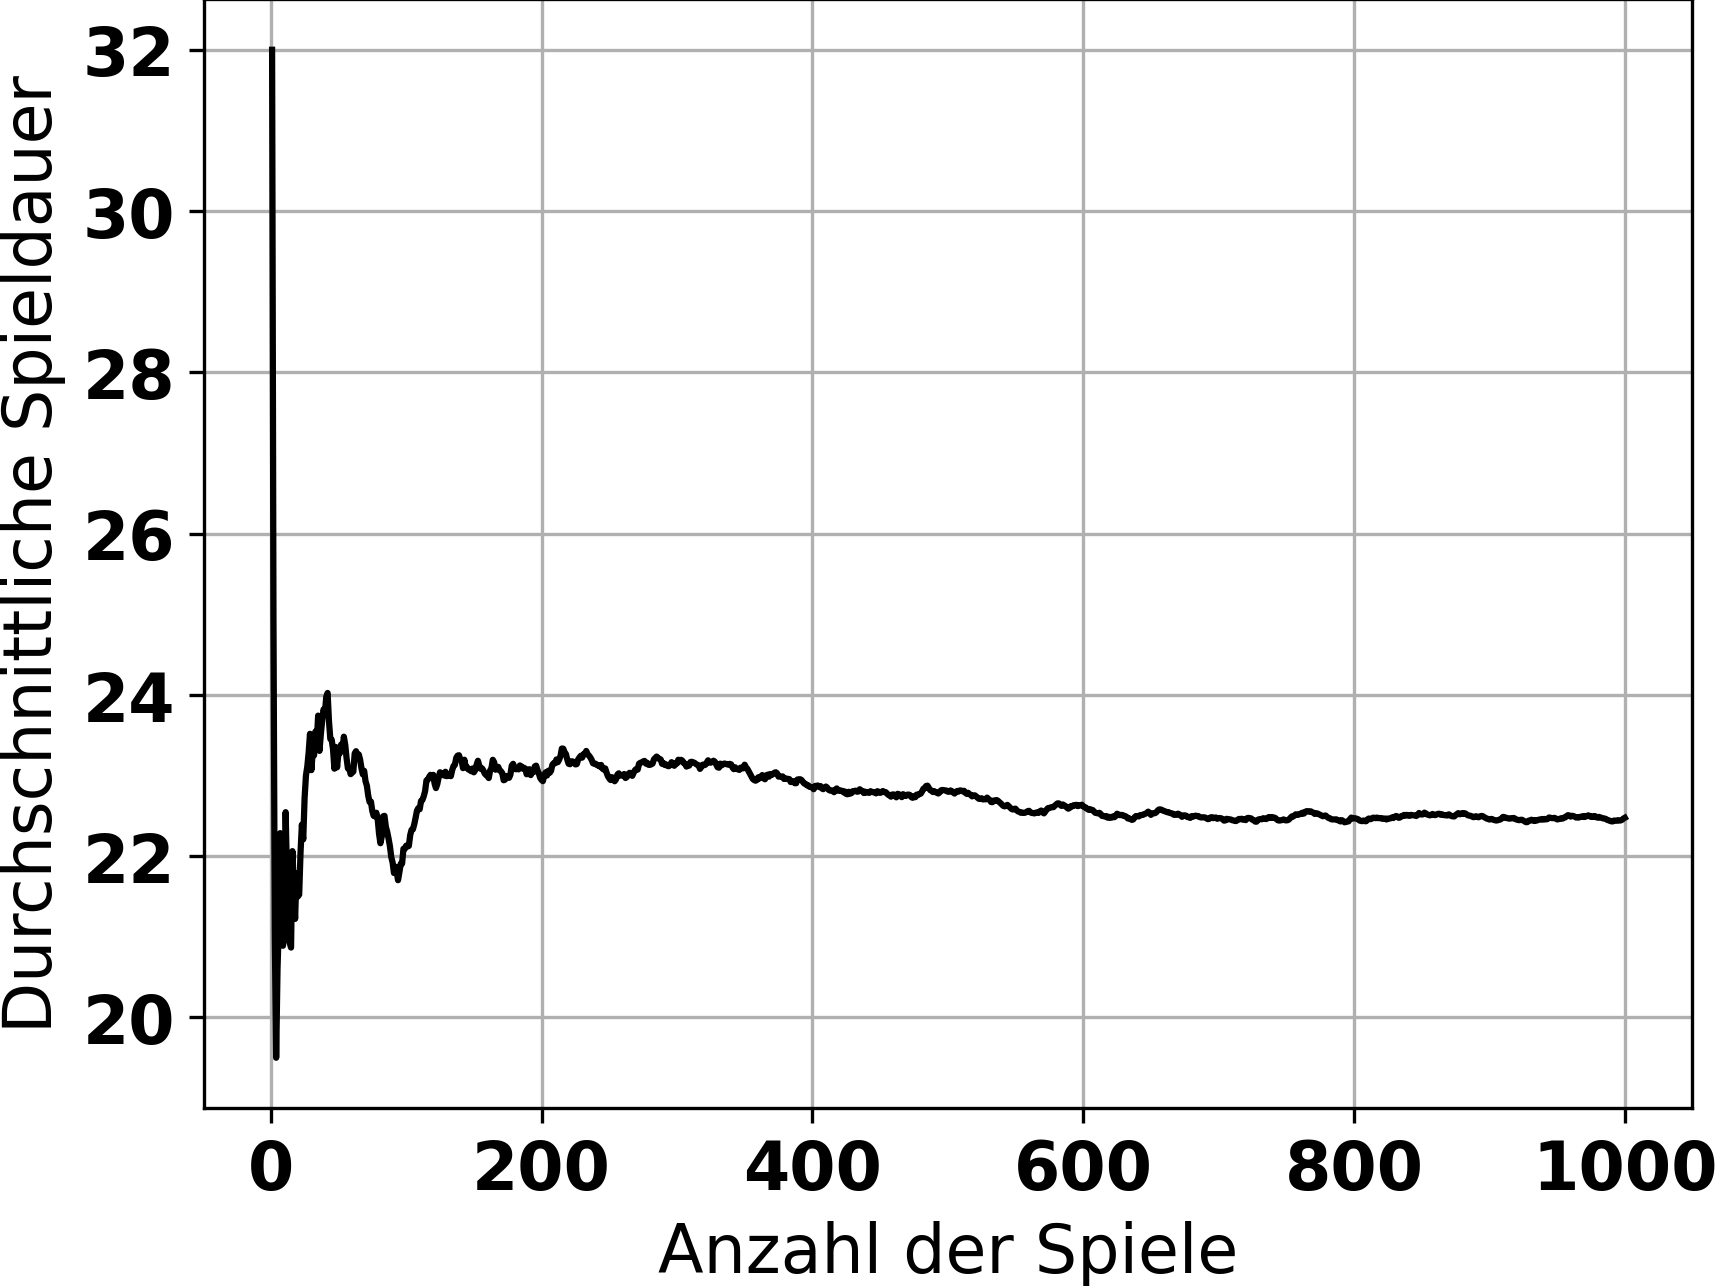
\includegraphics[width=\textwidth]{Bilder/constant_player_order_graph_game_length.png}
		\caption{Durchschnittliche Spieldauer.}
		\label{fig:f2}
	\end{subfigure}
	\caption{Gewinnrate und durchschnittliche Spieldauer bei konstanter Spielerreihenfolge.}
\end{figure}

Das lässt sich dadurch erklären, dass die Vier-Gewinnt-Umgebung so implementiert ist, dass Spieler 0 immer der Spieler ist, der den ersten Stein setzen darf. Er ist damit seinem Gegenspieler immer einen Spielzug voraus, was die Wahrscheinlichkeit erhöht, als erstes Vier Steine in eine Reihe zu bekommen. An dieser Stelle sei nochmals zu erwähnen, dass bei Vier Gewinnt der erste Spieler bei optimaler Spielweise stets gewinnen kann. Um ausgeglichene Messungen zu gewährleisten, muss daher sichergestellt werden, dass sich im Rahmen der Messungen die beiden Spieler mit dem ersten Zug abwechseln.

Die Vier-Gewinnt-Umgebung von PettingZoo wurde daher erweitert, um einen Parameter entgegenzunehmen und zu verarbeiten, der bestimmt, welcher Spieler anfangen soll. Die Messumgebung wechselt den Wert des Parameters nach jedem Spiel durch. Nach dieser Änderung weisen die Spiele wesentlich ausgeglichenere Ergebnisse auf. Spieler 0 gewinnt 50,30 \% und Spieler 1 49,50 \% der Spiele. Die durchschnittliche Spieldauer bleibt dabei mit 22,48 Zügen vor der Änderung gegenüber 22,26 Zügen nach der Änderung nahezu unverändert.

\begin{figure}[ht!]%[!tbp]
	\begin{subfigure}[b]{0.48\textwidth}
		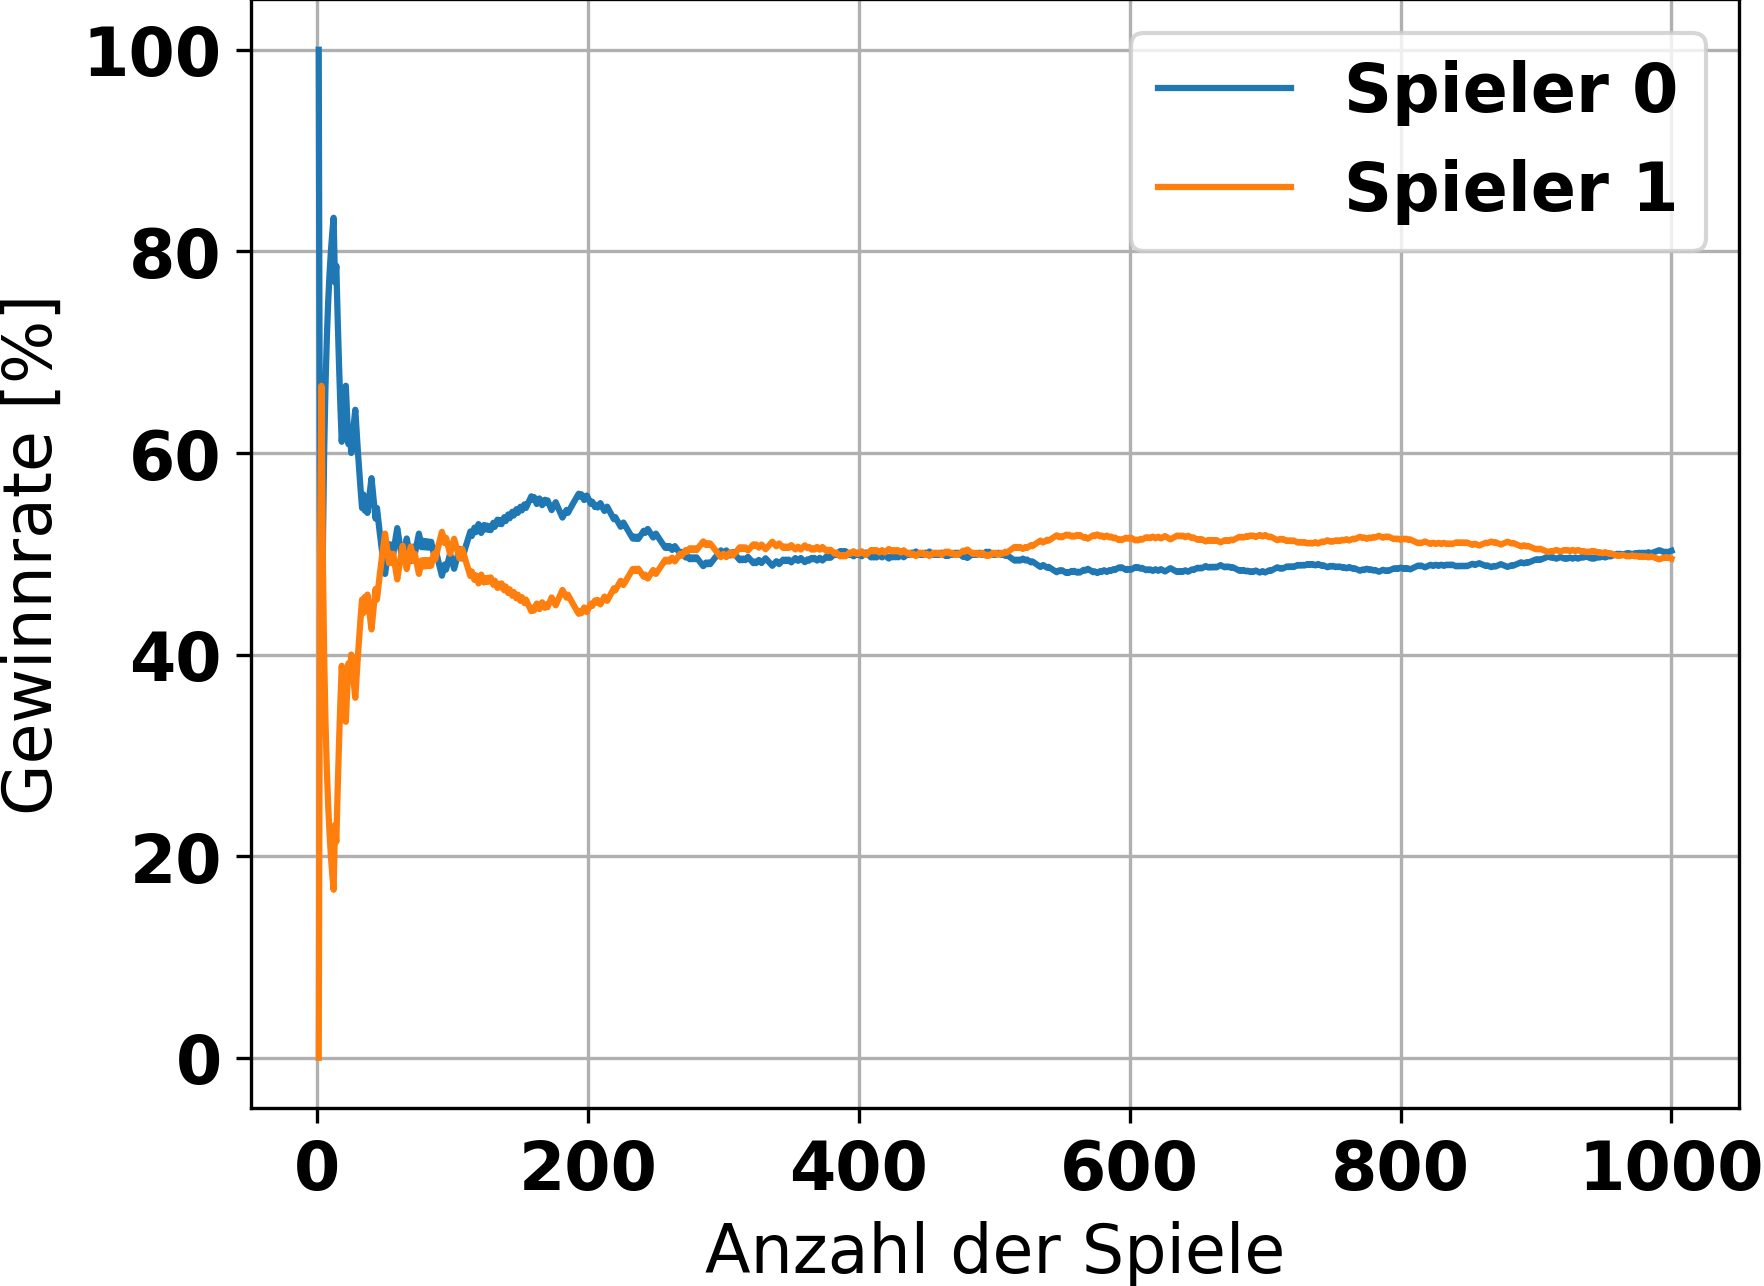
\includegraphics[width=\textwidth]{Bilder/alternating_player_order_graph_win_rates.png}
		\caption{Gewinnrate.}
		\label{fig:f3}
	\end{subfigure}
	\hfill
	\begin{subfigure}[b]{0.48\textwidth}
		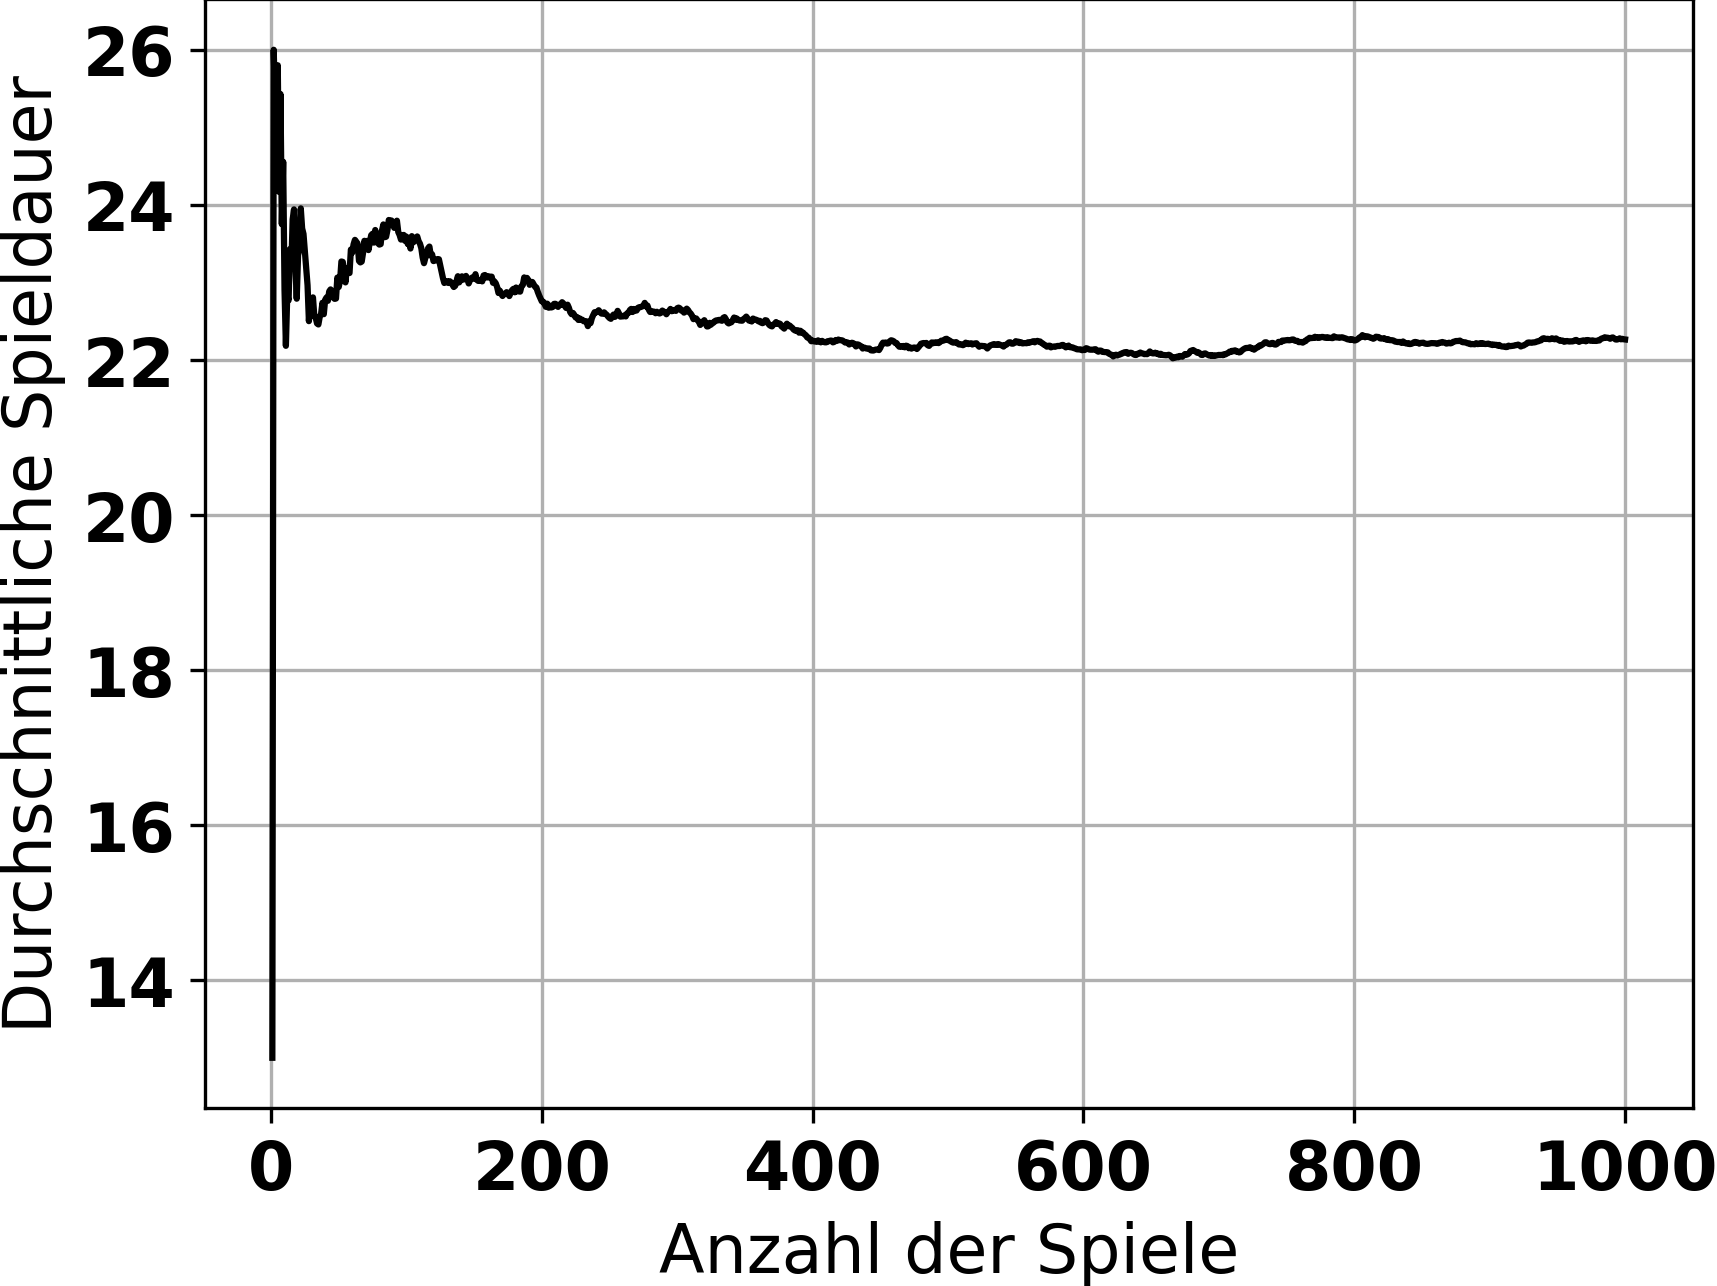
\includegraphics[width=\textwidth]{Bilder/alternating_player_order_graph_game_length.png}
		\caption{Durchschnittliche Spieldauer.}
		\label{fig:f4}
	\end{subfigure}
	\caption{Gewinnrate und durchschnittliche Spieldauer bei abwechselnder Spielerreihenfolge.}
\end{figure}



\subsection{MCTS-Agent}

Bei der Implementierung des MCTS-Agenten, diente \glqq Deep Learning and the Game of Go\grqq{} (\cite{Ferguson.January2019}, Kapitel 4.5) als Orientierung. Wie im genannten Werk besteht die im Rahmen dieser Arbeit entstandenen Implementierung aus zwei Klassen. Einer Klasse \texttt{MctsNode}, die einen Knoten im MCTS-Baum abbildet, und einer weiteren Klasse \texttt{MctsAgent}, die den Agenten repräsentiert und die wesentliche Logik des Algorithmus beinhaltet.

Die Klasse \texttt{MctsNode} besitzt dabei unter anderem folgende Attribute:
\begin{itemize}
\item \texttt{parent: MctsNode} und \texttt{children: list[MctsNode]}: Sie verwalten Beziehungen zu anderen Instanzen der Klasse \texttt{MctsNode}, sodass sie zusammen den MCTS-Baum abbilden.
\item \texttt{visitation\char`_count: int } und \texttt{total\char`_reward: int}: Diese Werte werden zur Berechnung der UCT-Werte in der Selection-Phase benötigt und in der Backpropagation-Phase aktualisiert.
\item \texttt{state: numpy.ndarray(6, 7, 2)}: Dabei handelt es sich um den Spielfeldzustand, den der Knoten repräsentiert. Das Format ist dabei dasselbe wie das, mit dem PettingZoo Beobachtungen über das Spielfeld zur Verfügung stellt. Dieses Attribut dient als Ausgangspunkt für die zufälligen Simulationen.
\end{itemize}

Die zentrale Methode der Klasse \texttt{MctsAgent} ist die Methode \texttt{determine\char`_action(self, state: numpy.ndarray(6, 7, 2)) -> int}. Sie nimmt den Zustand des Spielfelds entgegen, führt den MCTS-Algorithmus durch und gibt eine Zahl zurück, die die Aktion widerspiegelt, die auf Grundlage des Algorithmus gewählt werden soll. Zunächst wird darin ein Objekt der Klasse \texttt{MctsNode} initialisiert, dessen \texttt{state}-Attribut der beobachtete Zustand \texttt{state} zugewiesen wird. Dieses Objekt stellt den Wurzelknoten des MCTS-Baums dar. Anschließend werden n mal folgende Methoden wiederholt, wobei n die Anzahl der pro Entscheidung durchzuführenden Simulationen ist, die über den Konstruktor der Klasse konfiguriert werden kann:

\begin{itemize}
\item \texttt{select(root\char`_node: MctsNode) -> MctsNode}: Vom zuvor definierten Wurzelknoten werden per UCT-Formel solange Kinder ausgewählt, bis ein Knoten erreicht wurde, der ein Endzustand ist oder nicht vollständig expandiert ist, also weniger Kindknoten als Aktionen hat, die von dem dem Knoten entsprechenden Zustand möglich sind. Die UCT-Konstante kann dabei über den Konstruktor konfiguriert werden. Wenn es sich bei dem erreichten Knoten um einen Endzustand handelt, wird dieser Knoten zurückgegeben. Ansonsten, wird von diesem Knoten ein zufälliger legaler Spielzug ausgeführt und ein neuer Knoten, der den dadurch erreichten Zustand abbildet, wird als Kindknoten hinzugefügt. Dies entspricht dem Expansion-Schritt des MCTS-Algorithmus. Zurückgegeben wird dann der neu hinzugefügte Knoten.
\item \texttt{simulate(selected\char`_node: MctsNode) -> int}: Diese Methode nimmt den in der \texttt{select}-Methode ausgewählten Knoten entgegen, das Spiel wird ab dem Zustand, den der Knoten repräsentiert, zu Ende gespielt, und das Ergebnis des Spiels wird zurückgegeben.
\item \texttt{backpropagate(selected\char`_node: MctsNode, result: int) -> None}: Von ausgewählten Knoten wird das Attribut \texttt{visitation\char`_count} erhöht und das Ergebnis der Simulation zu \texttt{total\char`_rewards} addiert. Dieser Vorgang wird jeweils für alle Elternknoten durchgeführt, bis der Wurzelknoten erreicht wurde.
\end{itemize}

Nach n Wiederholungen wird eine Zahl zurückgegeben, die die Aktion repräsentiert, die vom Wurzelknoten zum direkten Kindknoten führt, dessen \texttt{visitation\char`_count}-Attribut den höchsten Wert hat.

% Anpassungen an der PettingZoo Umgebung

Für den Algorithmus wird ein Abbild für die Dynamik des Spiels benötigt, das unter anderem die Spielregeln, Gewinnbedingungen oder mögliche Aktionen in Abhängigkeit des aktuellen Zustands enthält. Dafür kommt in dieser Implementierung die Vier-Gewinnt-Umgebung von PettingZoo zum Einsatz. Diese enthält ein genau solches Abbild, und dadurch wird Aufwand in der Implementierung gespart. Es hat sich herausgestellt, dass an der Umgebung zwei Modifikationen notwendig sind, da die PettingZoo-Umgebungen in erster Linie zum Training von RL-Agenten konzipiert sind, und nicht um als Modell für symbolische Algorithmen oder modellbasierte RL-Verfahren zu dienen.

Zunächst wird keine Funktionalität unterstützt, um eine PettingZoo-Umgebung mit einem bestimmten Zustand zu initialisieren, was jedoch in der Klasse \texttt{MctsAgent} beispielsweise vor der Durchführung von Simulationen notwendig ist. Die Methode \texttt{reset(self, seed: int, options: dict) -> None} der Vier-Gewinnt-Umgebung wurde daher erweitert, um im \texttt{options}-Parameter nach dem Schlüssel \texttt{``state''} zu suchen, unter dem der gewünschte Zustand abgelegt werden kann, und ggf. entsprechend verarbeitet wird. Der Zustand wird dabei in derselben Form erwartet, wie PettingZoo seine Beobachtungen liefert.

Eine weitere Herausforderung bestand darin, dass PettingZoo-Umgebungen Beobachtungen stets perspektivisch aus Sicht des Agenten liefern, der aktuell am Zug ist. Im Fall von Vier Gewinnt bestehen die Beobachtungen aus einem Array, das das Spielfeld repräsentiert. Dieses Array enthält sechs weitere Arrays, die jeweils eine Reihe des Spielfelds abbilden, wobei jedes dieser Arrays sieben Felder enthält, die einem Feld in der jeweiligen Reihe entsprechen. Jedes dieser Felder ist ein Array bestehend aus zwei Elementen, die jeweils die Werte 0 und 1 annehmen können. Wenn das erste Element 1 ist, bedeutet das, dass der Spieler, der aktuell am Zug ist, einen Stein an der entsprechenden Position platziert hat. Wenn das zweite Feld 1 ist, bedeutet das, dass der Gegenspieler einen Stein platziert hat. 0 bedeutet, dass der entsprechende Spieler an der Position keinen Stein platziert hat \cite{Farama.2025}. Diese perspektivischen Beobachtungen erleichtern die Implementierung von RL-Agenten. Da die Vier-Gewinnt-Umgebung von PettingZoo jedoch nicht mit perspektivischen Beobachtungen, sondern mit einem globalen Zustand arbeitet, mussten Mechanismen implementiert werden, um diesen aus den perspektivischen Beobachtungen zu erzeugen. Dazu speichert die Klasse MctsNode, welcher Spieler als Nächstes am Zug ist, und die reset-Methode der Umgebung berücksichtigt einen entsprechenden Schlüssel im options-Parameter.

Aufgrund der zeitlichen Beschränkung dieser Arbeit wird auf Experimente bezüglich Optimierungen verzichtet. Daher wird als Auswahlstrategie in der Selection-Phase nach den Empfehlungen UCT mit $c=\sqrt{2}$ eingesetzt. Was die Expansion-Phase betrifft, wird sich ebenfalls an den Standard gehalten und nur einen und nicht mehrere Knoten hinzugefügt. In der Simulation-Phase werden Light-Playouts und keine Heavy-Playouts eingesetzt, da Light-Playouts ohne Wissen über das konkret zu lösende Problem auskommen, sodass die Ergebnisse dieser Arbeit so weit möglich auf verschiedene Probleme angewandt werden können.

\subsubsection{Zeitlicher Aufwand von Entscheidungen des MCTS-Agenten}

Die in dieser Arbeit durchgeführten Messungen fanden auf einem Computer mit einer Intel Core i7 8650U CPU statt. Ein MCTS-Agent, der pro Entscheidung 5.000 Simulationen durchführt, benötigt dabei für jeden Zug etwa eine zehn Sekunden. In einem Spiel mit einer Länge von 40 Zügen rechnet der MCTS-Agent also 3:20 Minuten. Für 200 Spiele, die im Rahmen dieser zeitlich begrenzten Arbeit an vielen Stellen als ausreichend für aussagekräftige Messungen betrachtet werden, werden für jeden beteiligten MCTS-Agenten 5 Stunden benötigt. Die Zeit steigt proportional zur Anzahl der durchgeführten Simulationen.

Es liegt nahe, den MCTS-Agenten durch Parallelisierung zu beschleunigen. Dadurch lässt sich die Rechenzeit proportional (ggf. sogar überproportional) zur auf der Maschine verfügbaren CPU-Ressourcen verkürzen, ohne dass die Ergebnisse dadurch beeinträchtigt werden (vgl. \cite{Chaslot.2008}). Dies ist vor allem bei Echtzeitanwendungen sinnvoll. Ein solcher Anspruch wird in dieser Arbeit jedoch nicht gestellt. Um die Komplexität des Algorithmus möglichst niedrig zu halten, wird auf die Parallelisierung von MCTS verzichtet. Stattdessen werden die Messungen parallelisiert und die Ergebnisse zusammengeführt.

\subsubsection{Quantitative Untersuchung}

% Da gehts morgen weiter.

\subsubsection{Qualitative Untersuchung}

Neben der quantitativen Analyse gegen zufällig spielende Agenten und gegen sich selbst wurde auch eine kurze qualitative Analyse im Spiel gegen einen menschlichen Spieler durchgeführt, um einen Eindruck über das Spielverhalten des MCTS-Agenten zu gewinnen. Der menschliche Spieler ist bei den Untersuchungen stets der Spieler, der den ersten Stein setzen darf. Er kann damit theoretisch jedes Spiel gewinnen und hat so mehr Kontrolle über den Spielverlauf, was die Analyse vereinfacht.

Ist der MCTS-Agent konfiguriert, um 500 Simulationen pro Entscheidung durchzuführen, lässt sich bereits beobachten, dass, wenn er bereits drei Steine in einer Kette platziert hat, stets den vierten Stein platziert, um zu gewinnen, sofern dies möglich ist. Wenn hingegen sein Gegenspieler drei Steine in einer Reihe hat, versäumt der Agent häufig, den vierten Stein zu blockieren, sodass der Gegenspieler das Spiel für sich entscheiden kann. Wird der MCTS-Agent nicht unter Druck gesetzt, wirken seine Züge häufig ziellos. Wenn er Angriffe vorbereitet, sind seine Züge leicht durchschaubar, was es als Mensch recht einfach macht, sie zu verteidigen. Es ist auch ohne strategische Kenntnisse des Spiels leicht möglich, gegen den MCTS-Agenten zu gewinnen. Ein Vorgehen das dabei häufig funktioniert, besteht darin, darauf abzuzielen, einen Stein in der vierten Reihe der mittleren Spalte platziert zu bekommen, und von dort aus eine diagonale Kette nach links unten oder rechts unten zu bilden. Manchmal geht dieser Plan nicht auf, jedoch entwickeln sich dadurch im Laufe des Spiels schnell andere offensichtliche Gewinnchancen.

Bei 2.500 Simulationen pro Entscheidung platziert der MCTS-Agent seinen ersten Stein meistens in der mittleren Spalte, sofern er frei ist, was laut Allis auch der stärkste Anfangszug ist \cite{Allis.1988}. Hat der Gegenspieler drei Steine in einer Kette positioniert, so wird diese Angriffsposition meistens durch den MCTS-Agenten verteidigt. Es macht sich auch bemerkbar, dass der Agent wesentlich aggressiver spielt. Platziert der Gegenspieler beispielsweise seine Steine zu Beginn des Spiels so, dass er keine Gefahr darstellt und die Bildung von Viererketten erst zum letztmöglichen Zeitpunkt verteidigt, baut der Agent Druck auf, sodass der Gegenspieler im restlichen Verlauf des Spiels häufig dazu gezwungen ist, einen bestimmten Zug zu wählen, um nicht im nächsten Zug zu verlieren. Verteilt der Gegenspieler seine ersten drei Steine auf die beiden gegenüberliegenden Ränder, erzeugt der Agent häufig eine Zwickmühle, in dem er seine ersten drei Steine jeweils in die unterste Reihe der drei mittleren Spalten platziert, sodass er im nächsten Zug gewinnen kann, indem er seinen Stein in der zweiten oder vorletzten Spalte platziert. Dieses Verhalten konnte bei 500 Simulationen nicht beobachtet werden. Auch hier gelingt die oben genannte Strategie, sich als Ziel zu setzen, eine Diagonale von einer unteren Ecke zur Position in der mittleren Spalte in der vierten Reihe zu bilden. Allerdings scheint der MCTS-Agent besser voraus zu planen, denn die Spiele dauern länger und sein Gegenspieler muss häufiger verteidigen.

Bei 5.000 Simulationen pro Zug setzt der MCTS-Agenten seinen ersten Stein, wenn möglich, stets in die mittlere Spalte. Es ist eine verstärkte Bildung von Zwickmühlen zu bemerken, sofern sie durch den Gegenspieler nicht frühzeitig erkannt und verhindert werden. Durch seine noch aggressivere Spielweise, ist es nur unter besonderer Anstrengung möglich, als menschlicher Spieler ohne Kenntnisse über die optimale Spielweise gegen den MCTS-Agenten zu gewinnen.

Meistens geschieht dies durch die Ausnutzung einer Schwachstelle, die der MCTS-Agent unabhängig von der Anzahl der Simulationen pro Entscheidung (auch bei 10.000 Simulationen) aufzuweisen scheint: Hat der Gegenspieler drei Steine in einer Kette platziert und es droht, dass er im nächsten Zug den vierten Stein platziert und damit das Spiel gewinnt, so blockiert der MCTS-Agent die Platzierung nicht in jedem Fall. Besonders deutlich wird dies, wenn der Gegenspieler drei Steine in einer Spalte aufeinander liegen hat, während der MCTS-Agent zwei Steine in einer anderen Spalte aufeinander liegen hat, und das Spielfeld ansonsten leer ist. Anstatt den Gegenspieler zu blockieren, setzt er häufig den dritten Stein in seine Spalte.

Um diese Schwachstelle weiter zu untersuchen, wurde der MCTS-Agent konfiguriert, um 10.000 Simulationen pro Entscheidung durchzuführen und es wurde mit verschiedenen Werten für $c_{UCT}$ gemessen, wie oft sich der MCTS-Agent in dieser Situation dafür entscheidet, den unmittelbaren Gewinn des Gegenspielers zu verhindern und wie oft er es bevorzugt, stattdessen den dritten Stein in seine Spalte zu platzieren und damit den Gewinn des Gegenspielers zuzulassen. Bei 200 Wiederholungen trifft der Agent stets eine der beiden Entscheidungen und entscheidet sich nie dafür, den Stein in einer anderen Spalte zu platzieren. Beim empfohlenen Wert von $c_{UCT} = \sqrt2$ entscheidet er sich mit einer Wahrscheinlichkeit von 20,0 \%, den Zug zu blockieren, bei $c_{UCT} = 1.7$ nur 5,5 \% und bei $c_{UCT} = 1.1$ sind es 44,0 \%. Je schwächer der Exploitation-Teil der UCT-Formel gewichtet wird, desto wahrscheinlicher wird es, dass der Agent den unmittelbaren Gewinn des Gegenspielers verhindert.

Eine mögliche Erklärung für dieses Verhalten besteht darin, dass in den vom MCTS-Agenten durchgeführten Simulationen alle Züge rein zufällig gewählt werden. So kann es passieren, dass für die Züge, die den Gegenspieler nicht blockieren, selten oder gar nicht der Fall eintritt, dass er unmittelbar darauf das Spiel für sich entscheidet. Gleichzeitig besitzt der Zug, der den dritten Stein in die Kette des MCTS-Agenten platziert, eine erhöhte Gewinnwahrscheinlichkeit. So steigt der UCT-Wert des entsprechenden Knotens im MCTS-Baum über den Exploitation-Teil der UCT-Formel, was dazu führt, dass dieser Zug in den Simulationen häufiger untersucht wird und am Ende mit einer höheren Wahrscheinlichkeit gewählt wird.

Bei einem geringeren Wert für $c_{UCT}$ werden Knoten, die selten untersucht wurden, häufiger untersucht als Knoten, bei denen aus den bisherigen Simulationen eine höhere Gewinnwahrscheinlichkeit hervorgegangen ist, sodass für nicht-blockierende Züge häufiger der Fall eintritt, dass der Gegenspieler das Spiel im nächsten Zug gewinnt, wodurch sich die Gewinnrate und damit der Exploitation-Teil aller Züge, die nicht blockieren, sinkt, der blockierende Zug häufiger simuliert und damit letztendlich auch gewählt wird.

Eine mögliche Lösung zum Beheben dieser Schwachstelle besteht darin, während der Simulationen nicht alle Züge rein zufällig zu wählen, sondern die Wahrscheinlichkeit zu erhöhen, dass der Gegenspieler den vierten Stein in eine bereits existierende Dreierkette platziert, sofern dies möglich ist, sodass in den Simulationen nicht-blockierende Züge eine niedrigere Gewinnrate aufweisen und mit einer niedrigeren Wahrscheinlichkeit gewählt werden.

Da das Ziel dieser Arbeit nicht darin besteht, optimale Agenten zu entwickeln, und die Ergebnisse möglichst unabhängig von Optimierungen auf Vier Gewinnt sein sollen, wird diese Funktionalität nicht eingebaut. Aufgrund der zeitlichen Beschränkung dieser Arbeit können mögliche Nebenwirkungen von niedrigen Werten für $c_{UCT}$ nicht untersucht werden. Aus diesem Grund werden die anstehenden Messungen weiterhin mit dem Standardwert von $c_{UCT} = \sqrt2$ durchgeführt.


% Es kommen Reinforcement Learning Modelle zum Einsatz, die aus RL-Bibliotheken wie CleanRL oder Stable-Baselines bereitgestellt werden. Falls vorhanden, wird auf fertig implementierte Algorithmen zurückgegriffen.

\newpage